% Created 2019-06-17 lun. 19:09
\documentclass[11pt]{article}
\usepackage[utf8]{inputenc}
\usepackage[T1]{fontenc}
\usepackage{fixltx2e}
\usepackage{graphicx}
\usepackage{longtable}
\usepackage{float}
\usepackage{wrapfig}
\usepackage{rotating}
\usepackage[normalem]{ulem}
\usepackage{amsmath}
\usepackage{textcomp}
\usepackage{marvosym}
\usepackage{wasysym}
\usepackage{amssymb}
\usepackage{hyperref}
\tolerance=1000
\usepackage[frenchb]{babel}
\usepackage{titlesec}\newcommand{\sectionbreak}{\clearpage}
\usepackage{wrapfig}
\author{Valentin LEBOUVIER}
\date{Encadrant: Catherine DEZAN}
\title{Rapport de TAL: Behaviour Trees}
\hypersetup{
  pdfkeywords={},
  pdfsubject={},
  pdfcreator={Emacs 25.2.2 (Org mode 8.2.10)}}
\begin{document}

\maketitle
\tableofcontents



\section{Introduction}
\label{sec-1}
Le Behaviour Tree (BT) est un outil qui a été créé pour modéliser les intelligences artificielles dans les jeux vidéos mais il est également utilisé dans la robotique. Le but principal de ce TAL était de voir si il était possible de créer une série de TP pour des L2 informatique en s'appuyant sur cet outil pour apporter un peu de thème et d'intérêt aux TPs proposés.

Dans ce rapport, nous allons tout d'abord décrire ce que sont les BTs, puis voir des exemples de BTs basés sur PacMan et enfin expliquer les TPs que j'ai préparé.

\begin{figure}[htb]
\centering
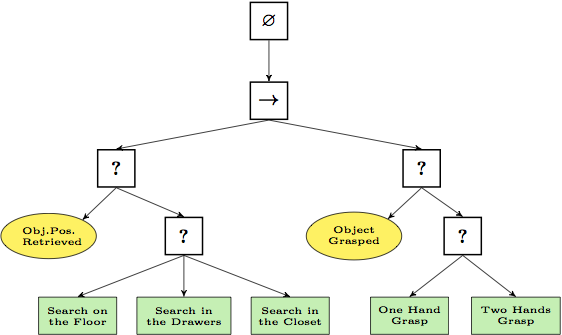
\includegraphics[width=0.85\textwidth]{./img/BT_search_and_grasp.png}
\caption{Exemple de BT}
\end{figure}

\section{Les Behaviour Trees (BTs)}
\label{sec-2}


Un Behaviour Tree (BT) est un outil permettant à un agent autonome de pouvoir choisir l'action à réaliser.
Il est utilisé pour créer des scénarios que suivront ces agents autonomes.
Il sert à la fois d'outil de conception et d'éxécution.
Le fait qu'il puisse être représenté graphiquement et même manipulé graphiquement dans certains environnements (Unity) en fait un outil très intuitif et rapide de compréhension.

Les BTs sont venus du besoin dans le monde du jeu-vidéo d'un outil de gestion des comportements plus performant que ceux qu'ils utilisaient.
Les BTs ont donc été créés dans le but de répondre aux problèmes de mission planning.
Ainsi, les BTs condensent certaines forces qui manquaient à d'autres outils.
Ainsi ses points forts sont sa modularité et sa réactivité, notions qui seront revues plus loin dans ce document. 

\subsection{Définition technique}
\label{sec-2-1}
\subsubsection{Définition}
\label{sec-2-1-1}
Un BT est un graphe orienté acyclique dont les noeuds retournent Succès, Échec ou En Cour selon les règles associées à ces noeuds.
Le status de chaque noeud est évalué par un \emph{tick} envoyé depuis la racine et qui parcourt le graphe selon les règles de parcours de chaque noeud.
Les noeuds ré-évaluent tous leurs enfants (selon leurs règles) à chaque fois qu'ils sont tickés.
Il y a de nombreuses définitions de ce que peuvent être les noeuds d'un BT.
Il faut aussi noter que dans certains modèles, un quatrième état peut être retourné par un noeud en cas de problème et retourner une exception.
La définition que je présente ci-après est celle de la bibliothèque py$_{\text{trees}}$ qui sera utilisée lors des TPs avec quelques modifications.
Ainsi il y a trois types de noeuds: les noeuds d'éxécution, les composites et les décorateurs.

\subsubsection{Les noeuds}
\label{sec-2-1-2}
\begin{enumerate}
\item Les noeuds d'éxécution
\label{sec-2-1-2-1}

Les noeuds d'éxécution sont les feuilles du BT, ce sont eux qui interagissent avec le modèle.

\clearpage
\begin{itemize}
\item Action:
\end{itemize}

\begin{figure}[htb]
\centering
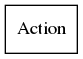
\includegraphics[width=0.3\textwidth]{./img/Action.png}
\caption{Noeud Action}
\end{figure}

Le noeud action retourne l'état dans lequel est l'action au moment du \emph{tick}.
L'action peut donc être en cours et retourner En Cours.
Elle peut être terminée correctement et retourner Succès.
Ou alors elle peut s'être terminée incorrectement et retourner Échec.

\begin{itemize}
\item Condition:
\end{itemize}


\begin{figure}[htb]
\centering

\includegraphics[width=0.3\textwidth]{./img/Condition.png}
\caption{Noeud Condition}
\end{figure}

Le noeud condition retourne l'état du test qui lui a été confié.
Ainsi la condition ne peut retourner que Succès si le test est vrai et Échec si le test est faux.

\item Les composites
\label{sec-2-1-2-2}

Les noeuds composites sont les noeuds de routage du BT, ils décident quelle branche prendre lors de l'évaluation du BT.
Les noeuds enfants sont toujours évalués du plus à gauche au plus à droite, sauf pour les noeuds parallèles qui les évaluent tous en même temps.
Les noeuds composites les plus courants sont les suivants:



\clearpage
\begin{itemize}
\item Séquence:
\end{itemize}


\begin{figure}[htb]
\centering
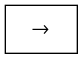
\includegraphics[width=0.3\textwidth]{./img/Sequence.png}
\caption{Noeud Séquence}
\end{figure}

Le noeud séquence n'évalue l'enfant suivant que si le précédent a retourné Succès, sinon il renvoie l'état de l'enfant courant.
Ainsi, ce noeud ne retourne Succès que si tous les enfants ont retourné Succès lors de ce \emph{tick}.

\begin{itemize}
\item Sélecteur:
\end{itemize}


\begin{figure}[htb]
\centering
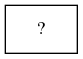
\includegraphics[width=0.3\textwidth]{./img/Selector.png}
\caption{Noeud Sélecteur}
\end{figure}

Le noeud sélecteur renvoie Succès dès qu'un enfant retourne Succès, sinon il retourne En Cours tant qu'il y a encore au moins un enfant qui retourne En Cours.



\clearpage
\begin{itemize}
\item Parallèle:
\end{itemize}


\begin{figure}[htb]
\centering
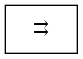
\includegraphics[width=0.3\textwidth]{./img/Parallel.png}
\caption{Noeud Parallèle}
\end{figure}

Le noeud parallèle envoie un \emph{tick} à tous ses enfants en même temps.
Le status qu'il renvoie dépend alors du nombre d'enfants qui retourne Succès ou Échec.
Les seuils M et N sont donnés à la création du noeud et représentent le nombre d'enfants devant retourner Succès (respectivement Échec) pour que le noeud parallèle retourne Succès (respectivement Échec).
Dans le reste des cas, le noeud retourne En Cours.

\begin{itemize}
\item Composites avec mémoire:
\end{itemize}


\begin{figure}[htb]
\centering
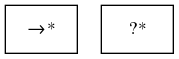
\includegraphics[width=0.6\textwidth]{./img/Memories.png}
\caption{Composites avec mémoire}
\end{figure}

Les noeuds composites avec mémoire fonctionnent comme leurs équivalents sans mémoire à l'exception prêt qu'ils se rappellent des résultats précédents donnés par les enfants.
Ainsi ils ne tickent pas les enfants qui ont déjà été évalués.


\clearpage
\item Les décorateurs
\label{sec-2-1-2-3}

\begin{figure}[htb]
\centering
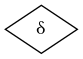
\includegraphics[width=0.3\textwidth]{./img/Decorateur.png}
\caption{Noeud décorateur}
\end{figure}

Les décorateurs sont des noeuds ne possédant qu'un seul enfant. Leur but est de modifier le résultat de cet enfant selon les règles que l'on choisit.
Pour donner quelques exemples tirés de la librairie:

\begin{itemize}
\item Inverter:
\end{itemize}

Ce décorateur inverse le résultat reçu de l'enfant, ainsi: Succès devient Échec, Échec devient Succès et En Cours ne change pas.

\begin{itemize}
\item Condition:
\end{itemize}

Ce décorateur attend un certain état de l'enfant pour passer à Succès, avant il retourne En Cours. 

\begin{itemize}
\item EternalGuard:
\end{itemize}

Ce décorateur met une condition sur l'éxécution d'un sous-arbre. Si la condition devient fausse, le sous-arbre se trouve arrêté.



\clearpage
\end{enumerate}
\subsection{Avantages des BTs}
\label{sec-2-2}
\subsubsection{Modularité}
\label{sec-2-2-1}
Pour qu'un BT soit modulaire, sa racine se doit de ne pas renvoyer Succès ou Échec lorsqu'il tourne mais seulement lorsqu'il a terminé tout ce qu'il avait à faire.
Cette modularité permet de pouvoir réutiliser ces BTs sans avoir à les redévelopper pour d'autres applications.

\subsubsection{Réactivité}
\label{sec-2-2-2}
La réactivité vient du fait que l'on puisse facilement interrompre une branche par une branche plus prioritaire (plus à gauche).
Cela permet de changer de comportement en un \emph{tick}.
Certains modèles de BTs permettent également de lancer un signal d'arrêt aux branches qui ont été interrompues.

\section{Exemple sur le PacMan}
\label{sec-3}
\subsection{Contexte}
\label{sec-3-1}
La création des BTs sur le PacMan vient du besoin de tester les BTs sur un exemple assez simple.
Et pour pouvoir tester ces BTs, un modèle de PacMan a été développé.
La plupart de ces BTs ont été développés et implémentés avec des noeuds séquence. Or il s'est avéré que les noeuds séquence de la librairie sont en fait des noeuds séquence avec mémoire.
Cela entraine que certains des premiers BTs ne fonctionnent pas exactement comme prévu mais le comportement reste tout de même proche de ce qui est attendu.

\subsection{Un PacMan Pas à Pas}
\label{sec-3-2}
Le premier BT réalisé permet de se déplacer dans le labyrinthe de façon "déterministe" (figure \ref{deterministe}).
C'est-à-dire que pour chaque direction il vérifie s'il y a un mur, s'il n'y en a pas le PacMan fait un pas dans cette direction.
L'ordre des directions ne changeant pas, le PacMan se retrouve donc toujours coincé dans un des coins du labyrinthe.

\begin{figure}[htb]
\centering
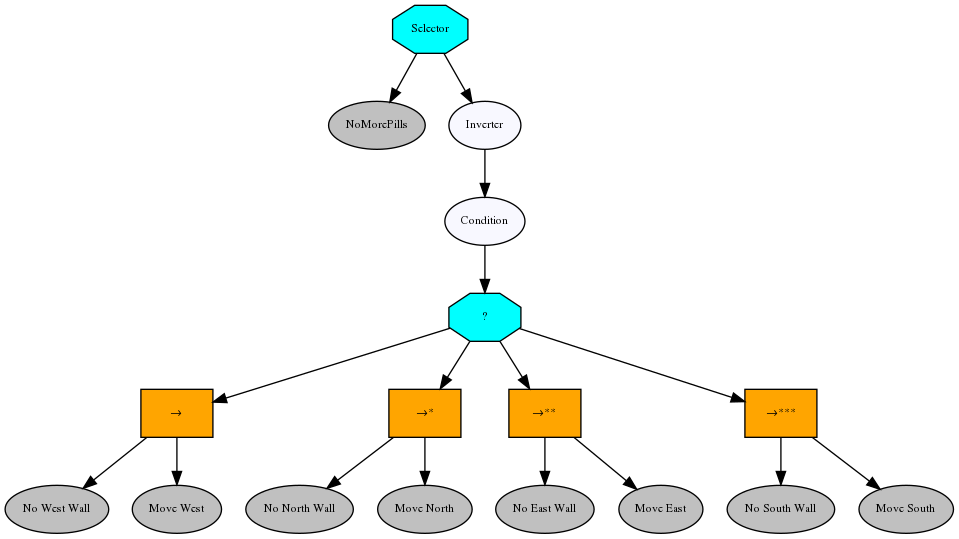
\includegraphics[width=.9\linewidth]{./img/PacManDeterministeBT.png}
\caption{\label{deterministe}PacMan déterministe}
\end{figure}


\clearpage
Un autre BT réalisé permet de choisir la direction dans laquelle se déplace le PacMan équiprobablement (figure \ref{equiprobable}).
Ainsi, PacMan a autant de chance de se déplacer dans chacune des cases adjacentes possibles.
Pour ce faire, la construction a été réalisée en suivant l'arbre binaire des possibilités de déplacement (figure \ref{schema_equiprobable})
Et pour chaque feuille de cet arbre binaire, faire un choix parmi les directions disponibles.

\begin{figure}[htb]
\centering
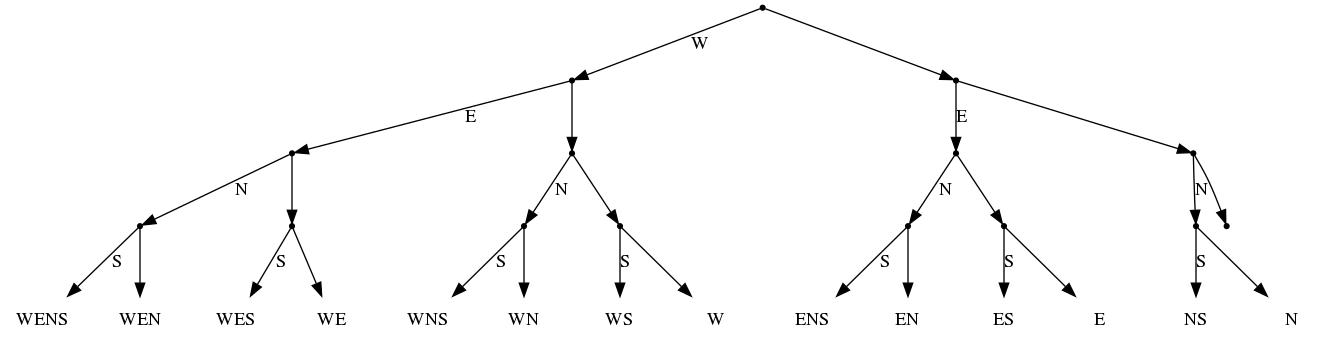
\includegraphics[width=0.8\textwidth]{./img/SimplifiedEquiprobable.png}
\caption{\label{schema_equiprobable}Arbre des possibilités de déplacement}
\end{figure}


\begin{figure}[htb]
\centering
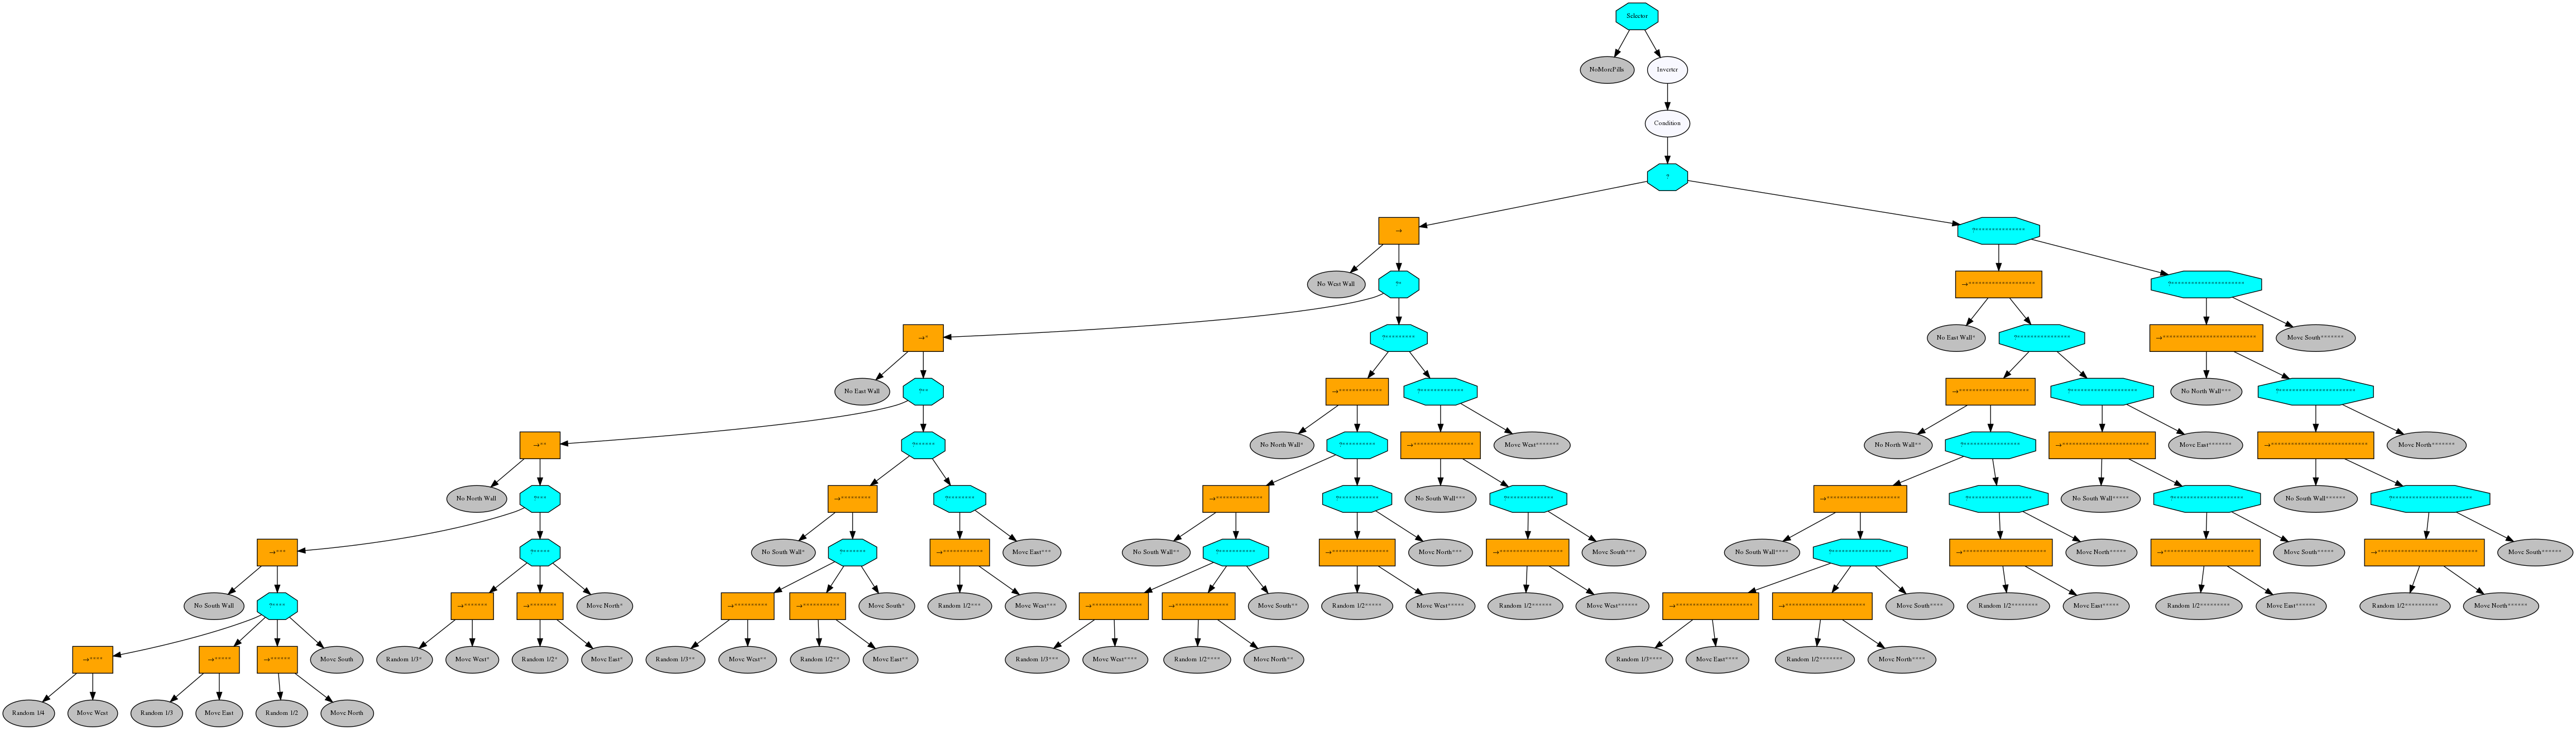
\includegraphics[width=.9\linewidth]{./img/PacManEquiprobableBT.png}
\caption{\label{equiprobable}PacMan équiprobable}
\end{figure}

\clearpage

Ces BTs possèdent une entête (figure \ref{entete}) permettant de filtrer les résultats indésirables (Succès) et de ne laisser remonter que les Échecs.
Pour ce faire, il y a un décorateur Condition qui se déclenche lors de la réception d'un Échec.
Cela renvoie donc un Succès qui est alors inversé pour récupérer un Échec. 

\begin{figure}[htb]
\centering
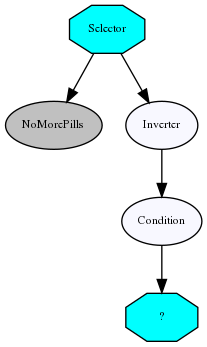
\includegraphics[width=0.25\textwidth]{./img/EnTete.png}
\caption{\label{entete}Entête PacMan}
\end{figure}

Le modèle (figure \ref{pacman_v0}) réalisé pour permettre l'éxécution de ces premiers BTs est des plus simples.
Il est composé principalement de tests pour savoir s'il y a des murs autour du PacMan, et de fonctions faisant se déplacer PacMan d'une case.

\clearpage
\subsection{Du Pas à Pas au Continu}
\label{sec-3-3}
Pour mieux simuler le comportement d'un PacMan, le modèle a été modifié pour accueillir des fantômes et faire en sorte que les déplacements soient continus (figure \ref{pacman_vf}).
Les BTs ne déplacent donc plus le PacMan mais lui disent dans quelle direction se diriger.
Ainsi il y a deux fonctions qui envoient périodiquement des ordres au modèle, une dans le BT qui actualise les directions de déplacement et une dans le modèle qui éxécute ces déplacements.
Cela a obligé à l'utilisation de threads, les deux fonctions étant bloquantes.

L'objectif avec ce nouveau modèle était de passer à un niveau d'abstraction plus haut pour le contrôleur et de se débarasser du contrôle direct des directions.
Pour ce faire les fonctions chase, gotoPill et flee ont été ajoutées ainsi que le principe de vision des autres personnages.
Le PacMan voit tous les fantômes (car il est supposé voir l'écran) alors que les fantômes ne voient PacMan que s'il passe dans le même couloir et se rapellent de la dernière position connue du PacMan en cas de perte de vision.
Pour éviter que le PacMan ne se fasse poursuivre à l'infini, les fantômes oublient la dernière position de PacMan au bout de 10 pas.
Pour pouvoir implémenter une recherche du plus court chemin pour gotoPill, un graphe du labyrinthe a été généré.

Plusieurs versions de BTs pour simuler une partie de Pacman ont été créés pour en arriver au BT suivant (figure \ref{bt_final}).
Malheureusement je n'ai pas réussi à trouver de façon rapide de faire fuir le PacMan, ainsi si il se trouve à moins de 10 cases d'un fantôme, il "panique" et se déplace aléatoirement.

\begin{figure}[htb]
\centering
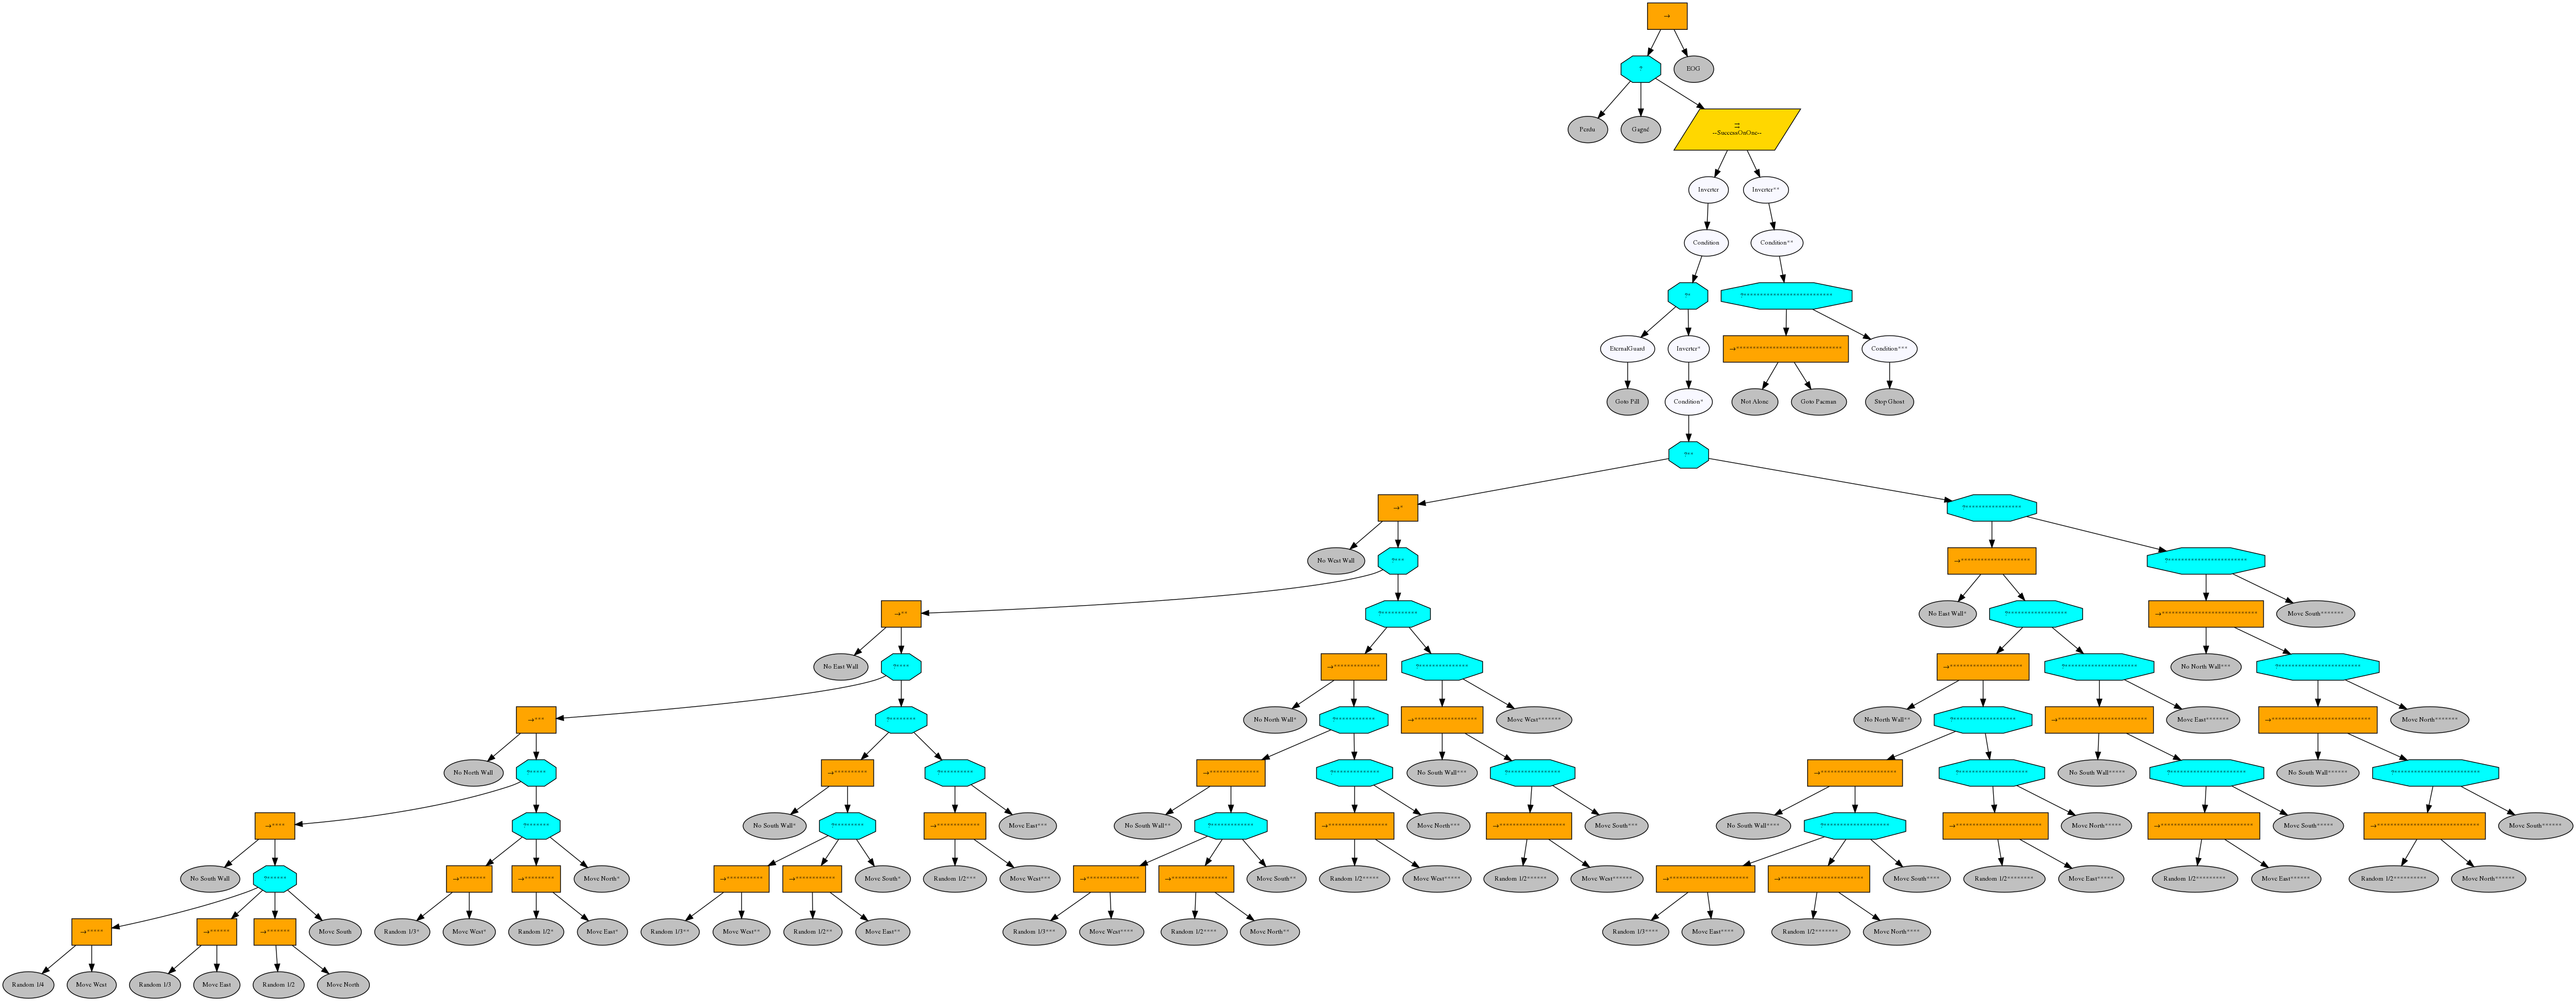
\includegraphics[width=.9\linewidth]{./img/LastPacMan.png}
\caption{\label{bt_final}BT continu}
\end{figure}

\clearpage
\subsection{Un PacMan Avec Interface}
\label{sec-3-4}
Pour rendre le PacMan plus lisible, une interface tkinter lui a été donnée. L'interface est passée d'un affichage textuel (figure \ref{texte}) à une fenêtre tkinter (figure \ref{tkinter}).
Cette interface demandant également une fonction bloquante pour fonctionner, elle a été d'abord mise dans un thread.
Or tkinter ne supporte pas très bien de ne pas tourner dans le thread principal, ainsi l'interface s'éxécute maintenant dans le thread principal et le contrôleur dans un autre thread.


\begin{figure}[htb]
\centering
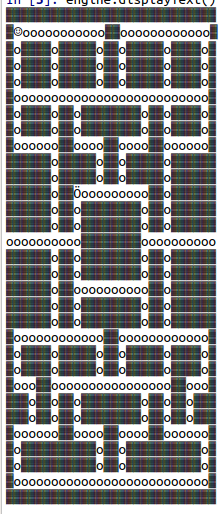
\includegraphics[width=.4\textwidth]{./img/AffichageTexte.png}
\caption{\label{texte}Ancien affichage}
\end{figure}


\begin{figure}[htb]
\centering
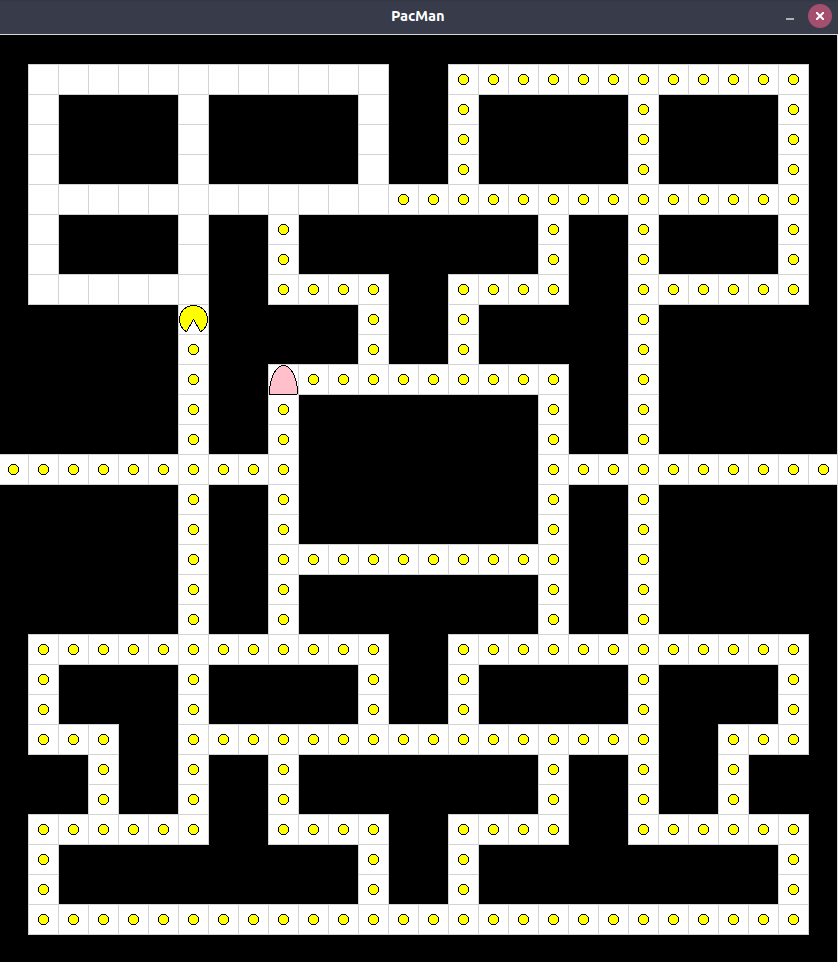
\includegraphics[width=.8\textwidth]{./img/PacMan.png}
\caption{\label{tkinter}Affichage tkinter}
\end{figure}



\subsection{Un Modèle MVC correct}
\label{sec-3-5}
Pour pouvoir proposer d'utiliser ce modèle dans les TPs, il a été modifié pour correspondre à un modèle MVC (Modèle-Vue-Contrôleur).
Ainsi plusieurs pattern Observateur ont été implémentés (figure \ref{pacman_vf}).


\section{TPs}
\label{sec-4}
\subsection{Rappel Contexte}
\label{sec-4-1}
Ces TPs seront donnés lors du cours de python lors du second semestre de L2 informatique.
Le but des TPs étant de familiariser les étudiants au language et à la Programmation Orientée Objet.
Les BTs ne sont là que pour apporter une structure plus intéressante et attirante pour les élèves grâce à un thème qui touche à l'Intelligence Artificielle, les jeux vidéo et la robotique. 
Les trames de ces 

\subsection{TP1 : Graphes \& BTs}
\label{sec-4-2}
Ce premier TP (figure \ref{TP1}) sert aux étudiants à se familiariser avec les graphes et à les manipuler en tant qu'objets python.
Le TP se déroulerait comme suit:
\begin{itemize}
\item Les étudiants ont un rappel sur les graphes et les parcours en profondeur
\item Les étudiants construisent une structure Noeud et écrivent la fonction qui leur permet de faire un parcours en profondeur
\item Les étudiants sont présentés aux BTs et sont conviés à créer un exemple simple avec py$_{\text{trees}}$
\end{itemize}

\subsection{TP2 : Tkinter}
\label{sec-4-3}
Ce second TP (figure \ref{TP2}) permet aux étudiants d'apprendre comment réaliser une interface avec tkinter.
Le TP se déroulerait comme suit:
\begin{itemize}
\item Les étudiants ont un cours sur tkinter (Tk, Frames, Widgets (Boutons,\ldots{}))
\item Les étudiants créent une première fenêtre toute simple (Tk \& un bouton pour fermer la fenêtre)
\item Les étudiants ont un petit cours sur les Canvas
\item Les étudiants mettent en place un Canvas pour afficher le background du PacMan
\end{itemize}

\subsection{TP3 : PacMan (MVC)}
\label{sec-4-4}
Ce dernier TP (figure \ref{TP3}) permet aux étudiants de découvrir ce qu'est le pattern MVC ainsi que des utilités plus poussées du Canvas
Le TP se déroulerait comme suit:
\begin{itemize}
\item Les étudiants sont présentés au PacMan via diagramme UML et on leur explique comment le modèle et le contrôleur fonctionnent
\item Les étudiants ont ensuite à réaliser la vue avec des indications du TP
\end{itemize}

\section{Conclusion}
\label{sec-5}

En ce qui concerne les BTs, ce sont des outils puissants de conception de scénarios pour des environnements où la prise de décision doit être rapide.

En ce qui concerne les TPs, un délai d'une semaine m'a été accordé pour finir l'écriture des TPs. Les documents en annexe ne sont que les trames plus ou moins complètes des futurs TPs.



\section{Annexes}
\label{sec-6}

\begin{figure}[htb]
\centering
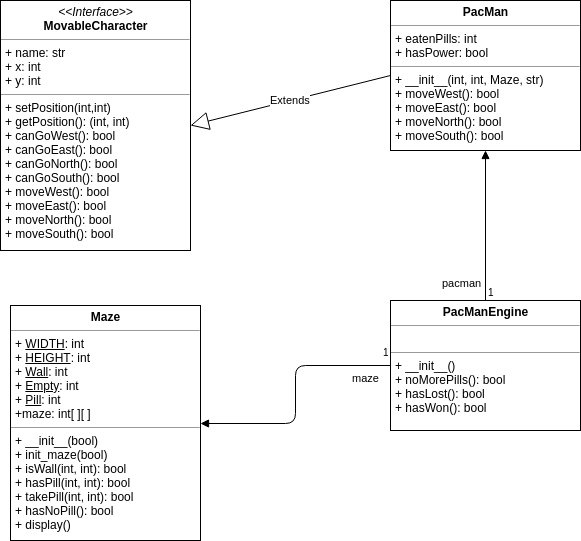
\includegraphics[width=.9\linewidth]{./img/Pacman_v0.png}
\caption{\label{pacman_v0}UML PacMan Pas à Pas}
\end{figure}

\begin{figure}[htb]
\centering
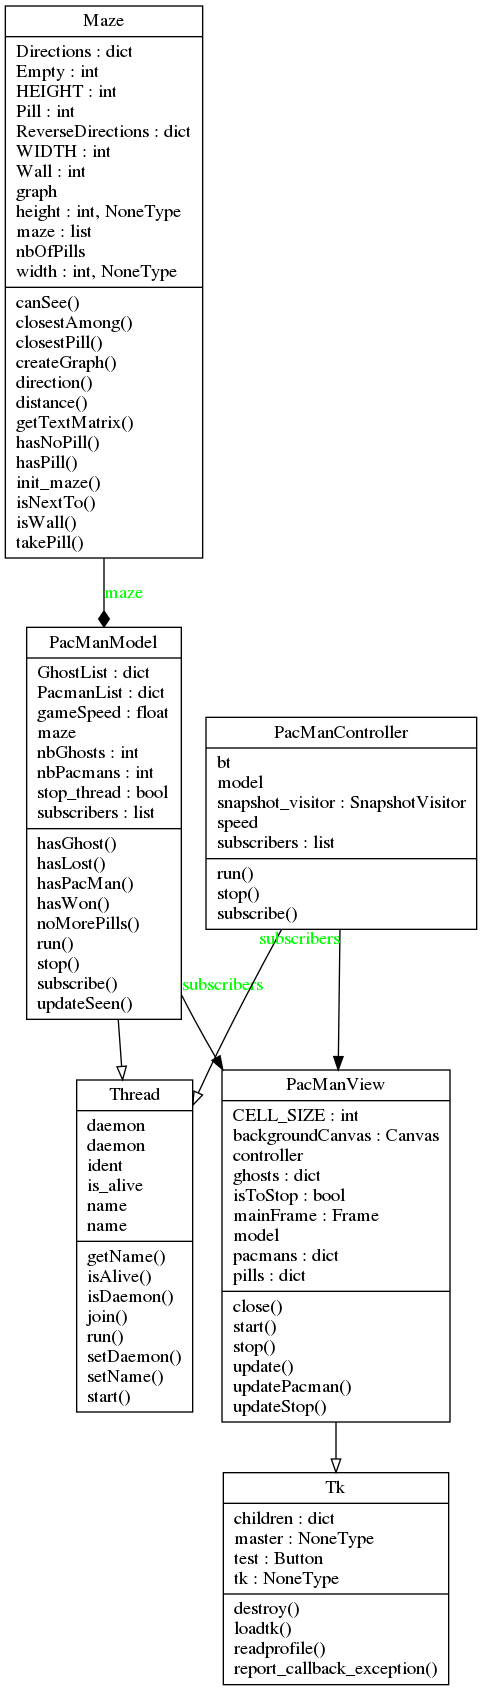
\includegraphics[width=.4\textwidth]{./img/Pacman_vf.png}
\caption{\label{pacman_vf}UML PacMan MVC}
\end{figure}

\begin{figure}[htb]
\centering
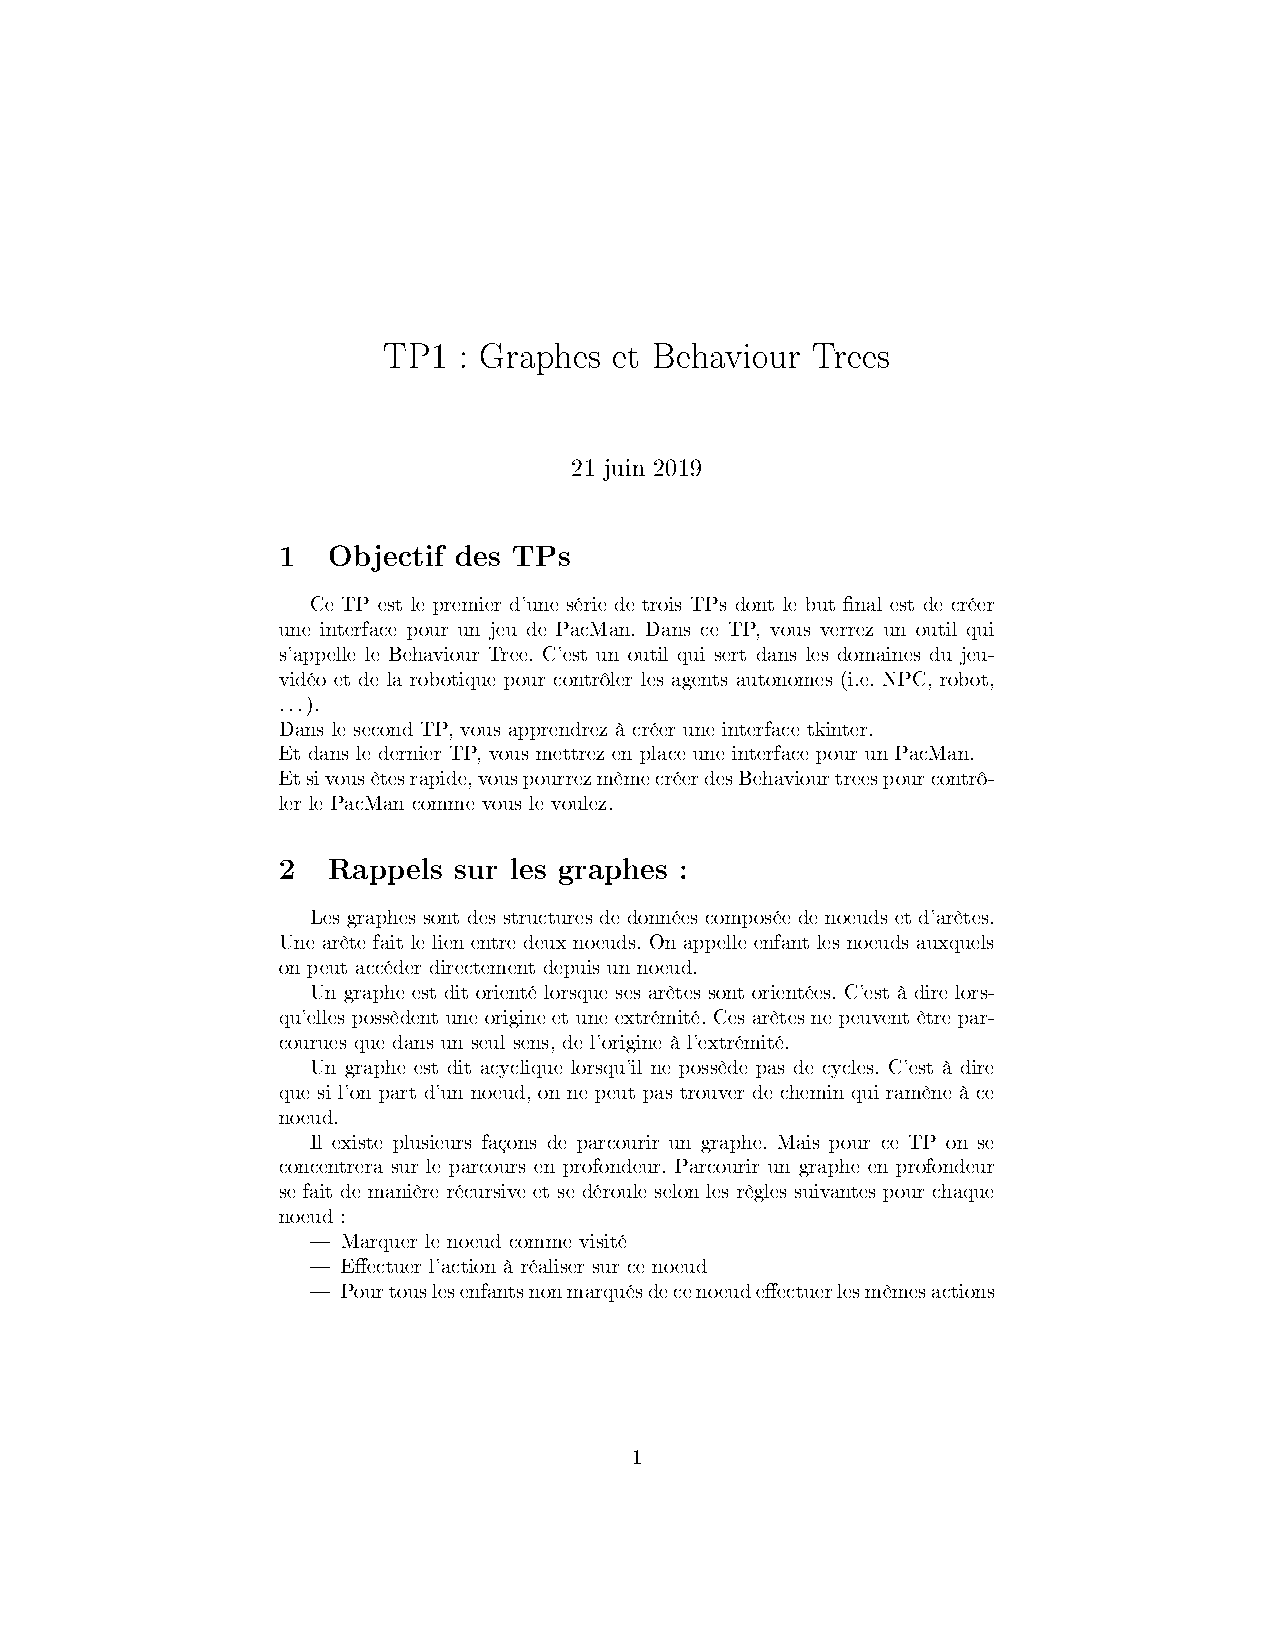
\includegraphics[width=.9\linewidth]{../TP/TP1/TP1.pdf}
\caption{\label{TP1}TP1}
\end{figure}


\begin{figure}[htb]
\centering
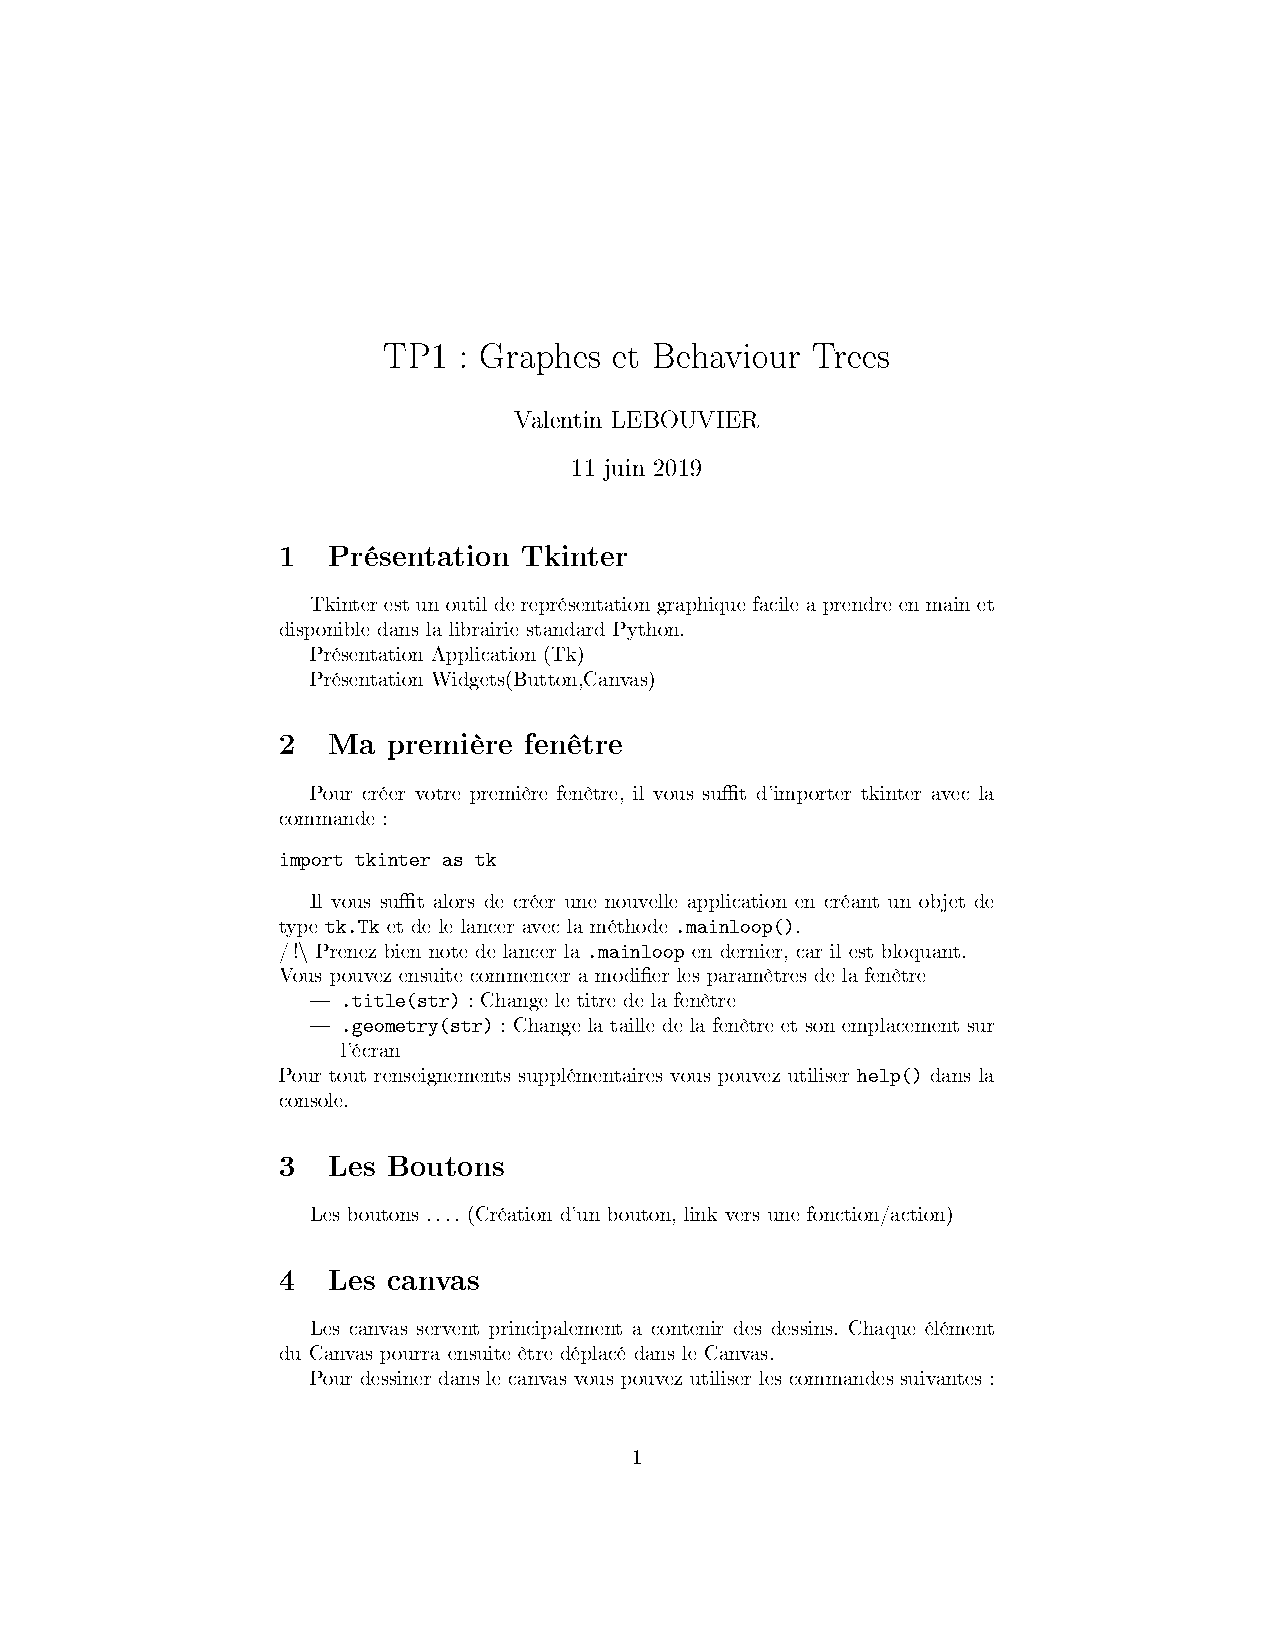
\includegraphics[width=.9\linewidth]{../TP/TP2/TP2.pdf}
\caption{\label{TP2}TP2 page 1/2}
\end{figure}


\begin{figure}[htb]
\centering
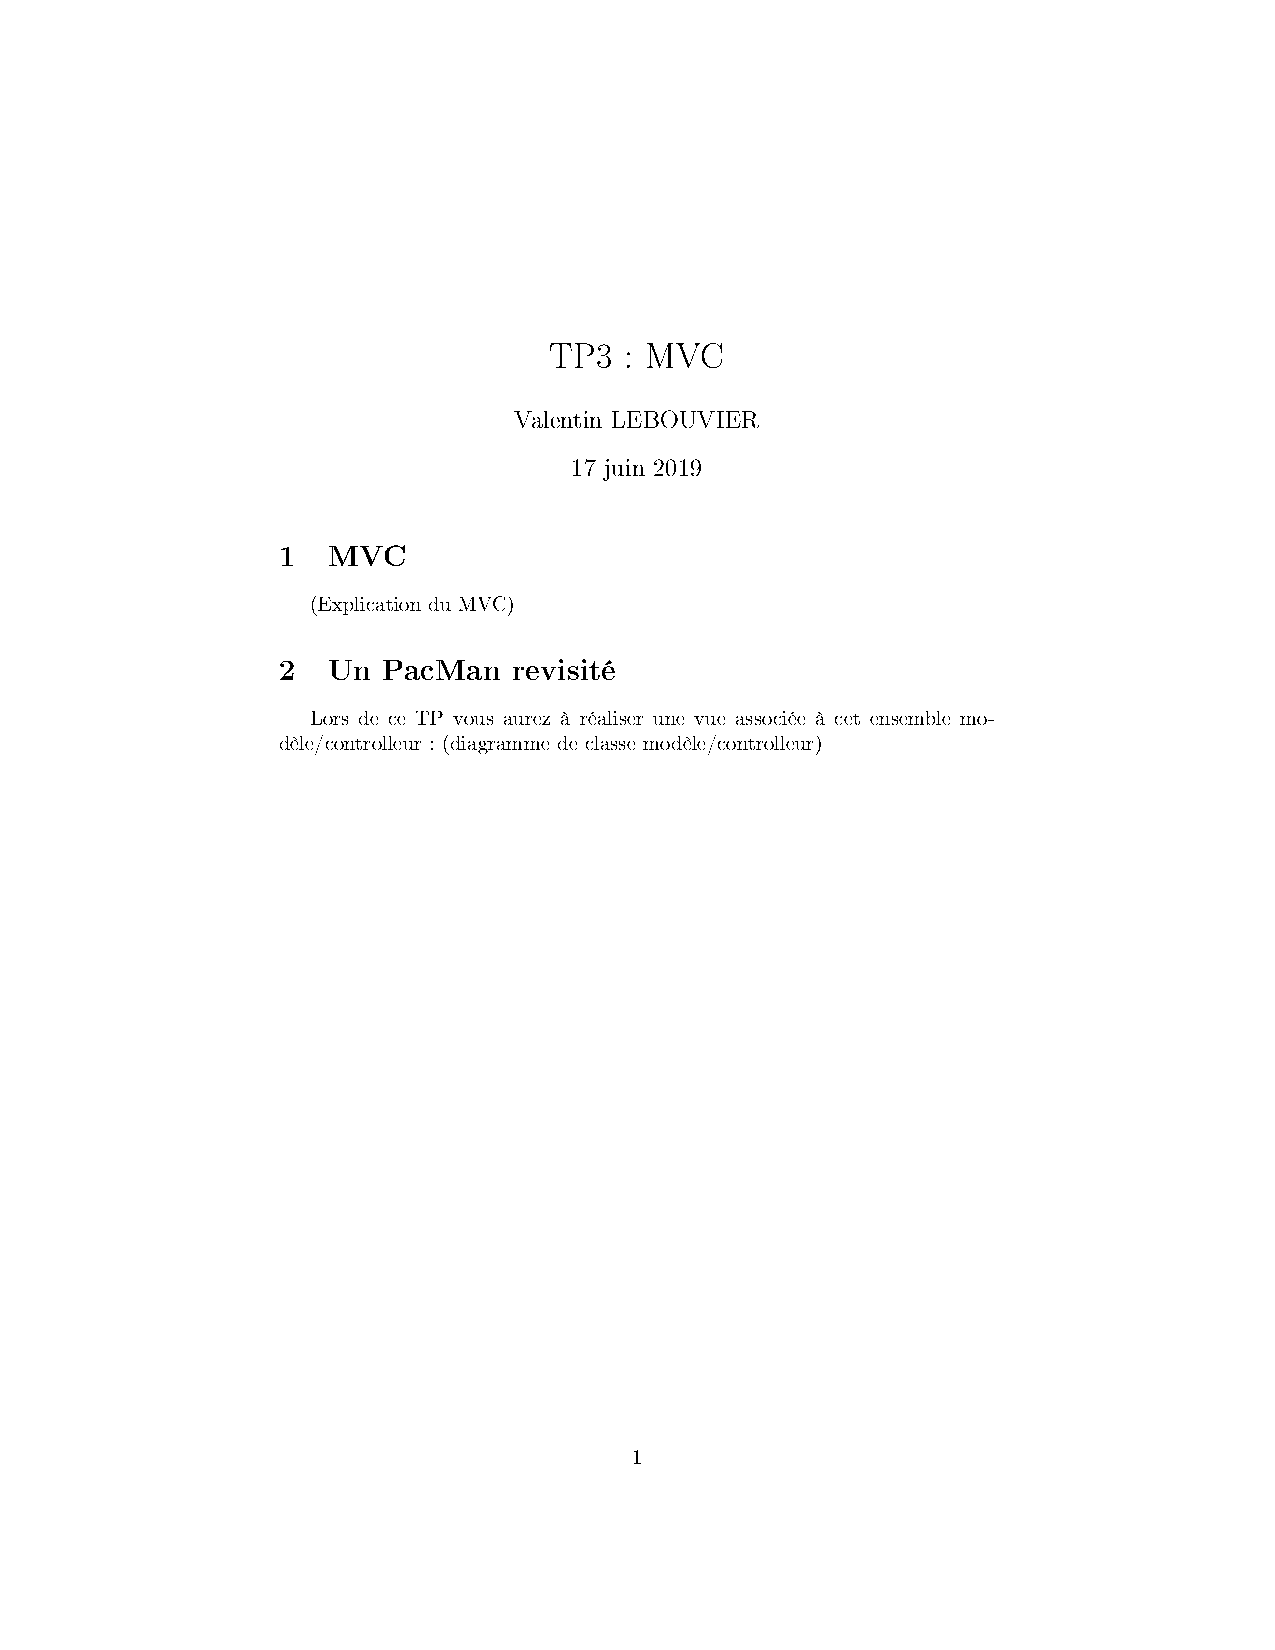
\includegraphics[width=.9\linewidth]{../TP/TP3/TP3.pdf}
\caption{\label{TP3}TP3}
\end{figure}
% Emacs 25.2.2 (Org mode 8.2.10)
\end{document}